\chapter{Puente de Wheatstone}

Los puentes de Wheatstone son los acondicionadores de señal para sensores resistivos más empleados. Consiste en dos divisores de tensión donde la tensión de salida se mide como la diferencia entre los dos potenciales, obteniéndose así el beneficio del rechazo al modo común y eliminación del offset. Si el puente está bien diseñado, esto es, se encuentra equilibrado, en ausencia de la magnitud a medir, la salida será $V_o = 0 V$.

\begin{itemize}
    \item Configuración 1 elemento sensible.
    \begin{figure}[H]
        \centering
        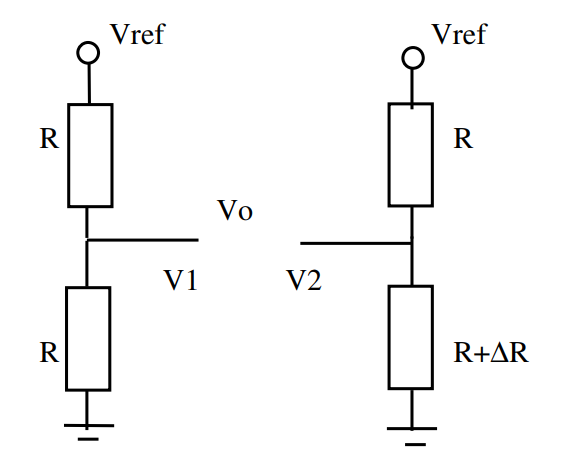
\includegraphics[width=0.4\linewidth]{Imagenes/Puente de Wheatstone 1.png}
        \caption{Puente de Wheatstone: 1 Elemento Sensible}
        \label{fig:wheatstone-1}
    \end{figure}
    
    \[V_o = V_{ref} \left( \frac{R + \Delta R}{2R + \Delta R} - \frac{1}{2} \right) = V_{ref}  \left( \frac{2R + 2\Delta R - 2R - \Delta R}{4R + 2 \Delta R} \right) = V_{ref}  \frac{\Delta R}{4R + \frac{4 \Delta R}{2}} \]
    
    Obteniendo finalmente:
    \begin{equation}
        V_o = V_{ref} \frac{\Delta R}{4R} \frac{1}{1 + \frac{\Delta R}{2R}}
    \end{equation}
    
    Donde se observa que si \(\frac{\Delta R}{2R} \ll 1\) tenemos que:
    \begin{equation}
        V_o = V_{ref}  \frac{\Delta R}{4R}
    \end{equation}
    
    \item Configuración 2 elementos sensibles.

    \begin{figure}[H]
        \centering
        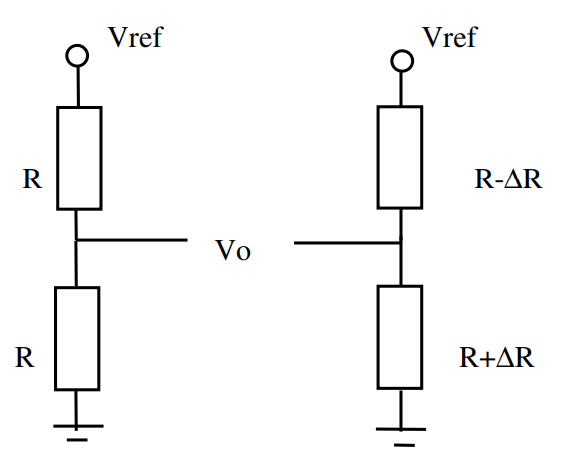
\includegraphics[width=0.4\linewidth]{Imagenes/Puente de Wheatstone 2.png}
        \caption{Puente de Wheatstone: 2 Elementos Sensibles}
        \label{fig:wheatstone-2}
    \end{figure}

    \[V_o = V_{ref}  \left( \frac{R + \Delta R}{R + \Delta R + R - \Delta R} - \frac{1}{2} \right) = V_{ref}  \frac{2R + 2 \Delta R - 2R}{4R} = V_{ref}  \frac{2\Delta R}{4R} \]

    \begin{equation}
        V_o = V_{ref}  \frac{\Delta R}{2R}
    \end{equation}
    
    \item Configuración 4 elementos sensibles.

    \begin{figure}[H]
        \centering
        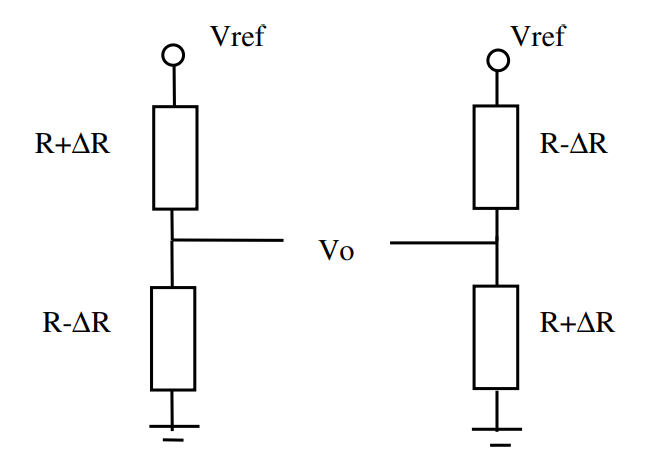
\includegraphics[width=0.4\linewidth]{Imagenes/Puente de Wheatstone 4.png}
        \caption{Puente de Wheatstone: 4 Elementos Sensibles}
        \label{fig:wheatstone-4}
    \end{figure}

    \[V_o = V_{ref}  \left( \frac{R + \Delta R}{R + \Delta R + R - \Delta R} - \frac{R - \Delta R}{R - \Delta R + R + \Delta R}\right) = V_{ref}  \frac{R + \Delta R - R + \Delta R}{2R} \]

    \begin{equation}
        V_o = V_{ref}  \frac{\Delta R}{R}
    \end{equation}
\end{itemize}

Se observa como mejoramos la sensibilidad al añadir más elementos sensibles, aunque también se encarece el montaje y aumenta la dificultad de conseguir elementos apareados. 

\section{Conexión remota}

Otra consideración referida a los puentes de Whetstone y aplicable a toda medida a distancia, consiste en la consideración de los hilos de conexión. Estos hilos implican la aparición de resistencias en serie al transductor. 

\begin{figure}[H]
    \centering
    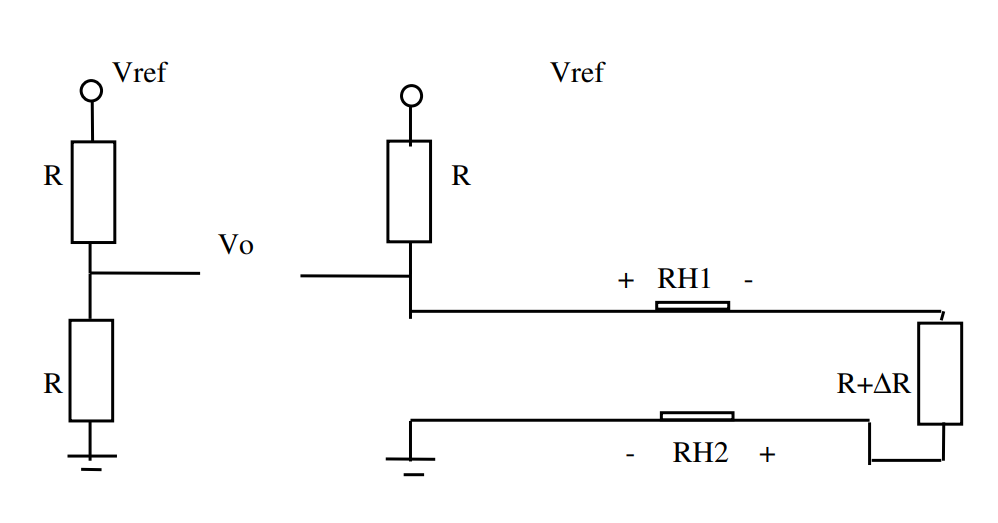
\includegraphics[width=0.5\linewidth]{Imagenes/Conexion 2 Hilos.png}
    \caption{Conexión incorrecta de un sensor resistivo a un puente remoto}
    \label{fig:2-hilos}
\end{figure}

Este problema se soluciona con el método de conexión de Siemens o de los tres hilos (Figura \ref{fig:3-hilos}). En esta configuración, los potenciales añadidos a $Vo$ por las resistencias de los hilos 1 y 2, se anulan, mientras que el potencial que añadiría la resistencia dle hilo 3, es despreciable pues, aunque exista resistencia, no circula corriente apreciable ya que se supone una alta impedancia de entrada del amplificador al que conectemos $Vo$.

\begin{figure}[H]
    \centering
    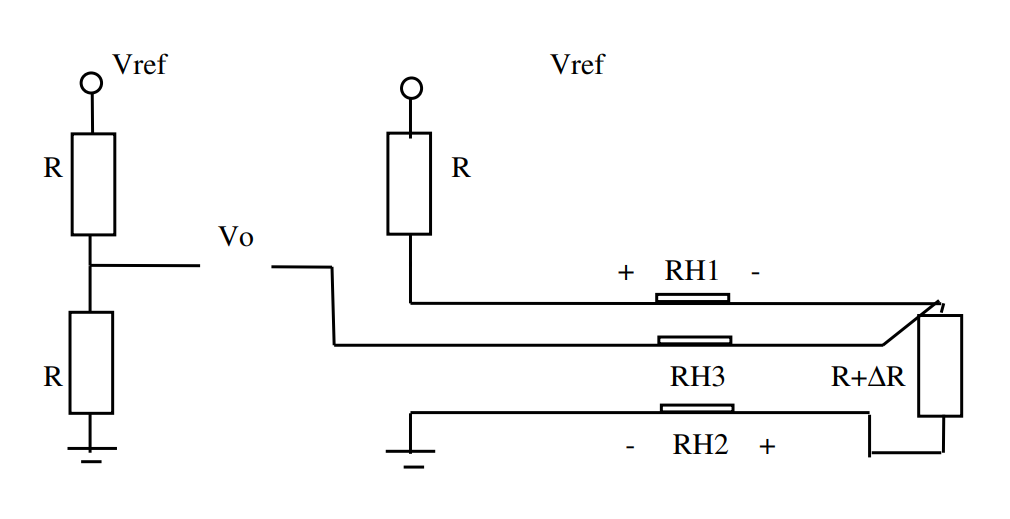
\includegraphics[width=0.5\linewidth]{Imagenes/Conexion 3 Hilos.png}
    \caption{Conexión de un sensor resistivo a un puente remoto: método de Siemens o de los tres hilos}
    \label{fig:3-hilos}
\end{figure}

\section{Ejemplo de aplicación: Anulación del efecto de la temperatura en galgas extensiométricas}

Para realizar medidas de fuerza con galgas extensiométricas, se disponen una o varias galgas en configuración de puente de Wheatstone. Para ello se utilizan galgas pasivas (Figura \ref{fig:galga-pasiva}), que son galgas iguales a las de medida dispuestas junto a ellas para que experimenten los mismos cambios de temperatura, pero que no están sometidas a esfuerzo porque se colocan transversalmente al mismo.

\begin{figure}[H]
    \centering
    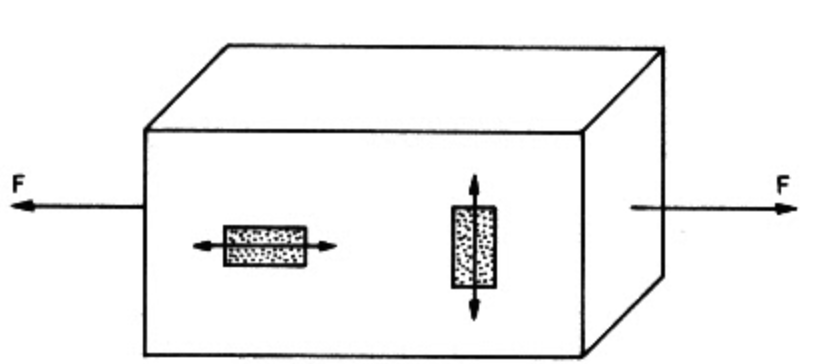
\includegraphics[width=0.5\linewidth]{Imagenes/Galga Activa y Pasiva.png}
    \caption{Galga pasiva}
    \label{fig:galga-pasiva}
\end{figure}
\begin{itemize}
    \item Configuración 2 elementos sensibles.

    \[V_o = V_{ref} \left( \frac{R (1 + \epsilon F)  (1 + \alpha \Delta T)}{R (1 + \epsilon F) (1 + \alpha \Delta T) + R (1 + \alpha \Delta T)} - \frac{1}{2} \right) = \]
    \[= V_{ref} \frac{2 + 2 \epsilon F - 1 - \epsilon F - 1}{2(1 + \epsilon F) + 2} = V_{ref} \frac{\epsilon F}{2(2 + \epsilon F)}\]

    Si \(2 \gg \epsilon F\) tenemos finalmente que:
    \begin{equation}
        V_o = V_{ref} \frac{\epsilon F}{4}
    \end{equation}

\end{itemize}